%% Synthesis Metapaper for Science
%% Algorithmic Objectivity for Congressional Redistricting

\documentclass[11pt]{article}

% Science journal style packages
\usepackage[utf8]{inputenc}
\usepackage[margin=1in]{geometry}
\usepackage{times}
\usepackage{amsmath,amssymb}
\usepackage{graphicx}
\usepackage{booktabs}
\usepackage{hyperref}
\usepackage{natbib}
\usepackage{tikz}
\usepackage{subcaption}
\usetikzlibrary{positioning,arrows.meta}

% Title and authors
\title{Algorithmic Objectivity for Congressional Redistricting: A National-Scale Demonstration}

\author{
Giovanni Della-Libera \\
\small Independent Researcher \\
\small \texttt{giodl73@gmail.com}
}

\date{\today}

\begin{document}

\maketitle

\begin{abstract}
Congressional redistricting in the United States suffers a legitimacy crisis:
partisan mapmakers manipulate district boundaries to predetermine election outcomes,
eroding public confidence in representative democracy. We evaluate recursive graph
bisection---a computational method used for supercomputer workload distribution---as a
partisan-input-excluded geographic benchmark. The execution stage does not consume
partisan data, but structure, weights, resolution, seed, and legal modifications remain
public policy choices. Historical pipeline runs cover all 50 states across three census
decades (2000/2010/2020) and produce population-balanced, contiguous district plans.
The demographic analysis reports majority-minority opportunity diagnostics, not legal
Voting Rights Act compliance; the reported 42\% threshold is exploratory rather than a
legal rule. Some ensemble and national headline claims still depend on synthetic or
incomplete evidence packages. The contribution is therefore a reproducible baseline and
research program, not proof of a uniquely fair map or a substitute for commissions,
courts, civil-rights analysis, or public judgment.
\end{abstract}

% Main sections
\section{The Redistricting Crisis}

Every ten years, American democracy faces a constitutional requirement with no constitutional solution: redrawing 435 congressional district boundaries to reflect population changes from the decennial census. This process, affecting 330 million Americans and determining electoral outcomes for a decade, suffers from a fundamental legitimacy crisis. Partisan legislatures manipulate district boundaries to predetermine election results---a practice known as gerrymandering---eroding public confidence in representative government~\cite{stephanopoulos2015partisan}.

The problem is ancient but newly precise. While gerrymandering dates to 1812, modern computing power enables manipulation with surgical accuracy~\cite{cho2016measuring}. Reformers have proposed independent redistricting commissions to remove partisan incentives, yet these still rely on human judgment about what constitutes ``fair'' districts. Even well-intentioned commissioners must balance competing values---compactness, community preservation, competitiveness---with no objective formula to guide their choices~\cite{duchin2018geometry}.

The legal landscape offers no remedy. In \emph{Rucho v. Common Cause} (2019), the Supreme Court ruled that partisan gerrymandering claims present ``political questions beyond the reach of federal courts,'' effectively removing federal oversight~\cite{rucho2019}. Chief Justice Roberts acknowledged the practice ``incompatible with democratic principles'' but declared courts institutionally incapable of policing it. This ruling created a governance vacuum: states may gerrymander with impunity, and no mathematical standard exists to distinguish legitimate from illegitimate maps.

This program is scoped to congressional and state-legislative redistricting. Local redistricting for city councils, school boards, and county commissions is outside the present research boundary.

We evaluate recursive graph bisection---a computational method developed for distributing workloads across supercomputer processors---as a reproducible geographic benchmark for redistricting. Applied to all 50 states across three census decades (2000, 2010, 2020), the historical pipeline produces population-balanced, contiguous plans while excluding partisan data from the benchmark execution inputs. This is an input-exclusion claim, not an impossibility theorem: structure, geographic resolution, weights, seed rules, and legally required modifications can affect political outcomes and can themselves be selected strategically. Compact benchmark maps can also reflect geographic voter concentration, as shown in Track C.5. The contribution is an auditable comparison procedure that can support commissions, courts, and public review rather than replace them.

\section{The Huntington-Hill Precedent}

Congressional redistricting is not the first time American democracy has confronted the need for algorithmic objectivity. For 150 years, Congress struggled with an analogous problem: apportioning House seats among states based on decennial census counts. From 1790 to 1941, every census triggered political battles over which mathematical method to use, with each formula favoring different states. Congress changed the apportionment method six times, always to advantage particular political coalitions~\cite{balinski1982fair}.

In 1941, Congress adopted the Huntington-Hill method of equal proportions, a
formula that has supplied a durable operational allocation rule for eight
decades~\cite{huntington1928methods}. The method did not end disputes over
House size, census counts, constitutional interpretation, or alternative
apportionment axioms. Its narrower achievement was to remove cycle-specific
allocation discretion after Congress selected the method and inputs.

This precedent suggests a pathway for redistricting. Just as apportionment answered ``How many seats per state?'' with mathematical objectivity, redistricting might answer ``Where to draw district boundaries?'' through algorithmic methods. The parallel is instructive:

\begin{center}
\begin{tabular}{ll}
\textbf{Apportionment (operational rule)} & \textbf{Redistricting (open rule)} \\
How many seats per state? & Where to draw boundaries? \\
Mathematical formula (1941) & Partisan negotiation \\
Durable post-enactment procedure & Persistent method and boundary conflict \\
\end{tabular}
\end{center}

The relevant question is whether Congress can create a similarly durable
post-enactment decision procedure for a harder problem while preserving legal
and representational judgment.

\section{Recursive Bisection Method}

Recursive graph bisection, originally developed for distributing computational
workloads across parallel processors~\cite{karypis1998metis}, can produce a
reproducible geographic benchmark for redistricting. The method represents a
state as a graph, balances population while partitioning the graph, and records
the resulting assignments and parameters for independent review.

\subsection{Benchmark Execution}

The historical national pipeline used census tracts as graph nodes and tract
population as the vertex weight. Edges connect units that share a published
geographic boundary. In the default geographic profile, the edge weight is the
shared-boundary length from the applicable TIGER/Line vintage. METIS minimizes
the weighted cut while recursively allocating the required number of districts.

This profile excludes election results, party registration, incumbency,
candidate identity, race, and community submissions from benchmark
generation. That exclusion is auditable from the configuration and manifest,
but it does not make the profile value-free. Tract resolution, recursive
structure, boundary weighting, population tolerance, random seed, and engine
version can all affect the output.

The governed operational profile is NRS v0.3. It uses 15-digit Census blocks,
versioned State adjacency contexts, a fixed floor/ceiling recursive seat
schedule, manifest-derived seeds, deterministic candidate refinement, and
one-based canonical district labels. For each Census cycle, the published
package binds the executable, input inventory, standard and legal profiles,
State assignment/tree manifests, national proof-coverage summary, and an
independent verification pass. NRS v0.3 is a later research profile; it does
not silently amend the v0.1 schedule incorporated by the candidate model
statute.

Race-conscious VRA-aligned weighting and partisan-weighted analysis are
separate research or case-specific profiles. They are not part of the default
geographic benchmark and must not be used to describe that benchmark as both
race-blind and VRA-compliant.

\subsection{Reproducibility And Configuration}

A reproducible run must identify:

\begin{itemize}
\item census and TIGER/Line releases;
\item geographic-unit index and adjacency definition;
\item district count and population source;
\item structure, edge-weight, search, and engine profiles;
\item balance settings and seed;
\item source commit, compiler, dependency lock, and binary provenance; and
\item canonical hashes linking assignments, analysis, and reports.
\end{itemize}

The current project supports several structures, weight signals, and search
modes. Results from one profile do not establish properties of another. The
candidate national-standard decision record selects standard recursive
bisection, geographic boundary weights, and one precommitted content-derived
seed as a comparison benchmark. Seed wiring and block-level operational
conformance are implemented and verified nationally in NRS v0.3. The earlier
tract outputs analyzed elsewhere in this paper remain separate research
artifacts; they are not NRS v0.3 certificates and cannot supply missing
demographic, partisan, or community evidence for the block-level assignments.
Geometric compactness is supplied only by the later precommitted 2020 bakeoff,
which dissolves NRS and official CD118 assignments over the same retained
Census-block polygons. It measures block-projected geometry rather than the
official plan's original polygon linework.

\subsection{Sequential Public-Cut Ceremony}

For a certified recursive plan, precommitment can be made observable rather
than merely asserted after completion. A genesis artifact binds the rule
profile, root instance, canonical floor/ceiling district tree, review interval,
witness threshold, and challenge policy. The root cut is published after one
review window; subsequent non-leaf cuts are released by tree depth and ordered
by binary path. Each release includes its split instance, certificate, proof,
timestamp, witness receipts, and prior-round hash.

The public verifier checks each disclosed prefix without access to unreleased
descendants, including exact parent-to-child universe derivation. Completion
binds the final certified tree; a sustained challenge instead leaves an
immutable halted transcript. The implementation checks receipt presence and
uniqueness, not an external service's signature or clock, so production claims
require separately validated transparency-log or trusted-timestamp adapters.

Prospective bakeoffs use a separate procedural scoreboard for proof coverage,
prefix verification, ceremony status, transcript size, verifier time, and
negative-test resistance. These fields are not blended with map-quality
metrics into a single winner. Existing bakeoffs remain governed by their
original frozen protocols and carry no retroactive ceremony claim.

\subsection{Population And Contiguity}

Population equality is reported as an observed property of each output, not as
a claim that one configured tolerance is always legally sufficient. For
congressional districts, the controlling legal principle is equality as nearly
exact as practicable. A complete evidence package must report ideal population,
maximum and total deviation, and any post-partition repair.

Contiguity is evaluated against the published adjacency graph. Water, islands,
point contacts, slivers, and bridge corrections can alter that graph and must be
versioned rather than silently repaired.

\subsection{Performance And Evidence Scope}

The Rust implementation makes national experimentation practical, but runtime
depends on state size, engine, data cache, profile, and search mode. Historical
benchmark tables in this paper are engineering measurements tied to their named
environment; they are not universal runtime guarantees.

Ensemble generation is distinct from producing one benchmark plan. A single
run can be reproduced and compared, but it cannot define the distribution of
valid alternatives. Ensemble percentile claims require archived real traces,
multiple chains, convergence diagnostics, immutable election inputs, and
uncertainty reporting.

\subsection{Input-Exclusion Defense}

The defensible procedural claim is narrow: a run whose manifest binds only
population and geographic inputs cannot directly target partisan outcomes
during execution using partisan data that it never receives. This is an
input-exclusion defense, not an impossibility defense.

Partisan consequences may still arise from political geography, and upstream
choices can be manipulated if they are selected after observing outcomes. A
credible standard therefore precommits assignment-affecting profiles, publishes
the benchmark, reports sensitivity, and discloses every baseline-to-final
modification. Human legal and community judgment remains necessary.


% Figures (generated PNG files)
\begin{figure}[t]
\centering
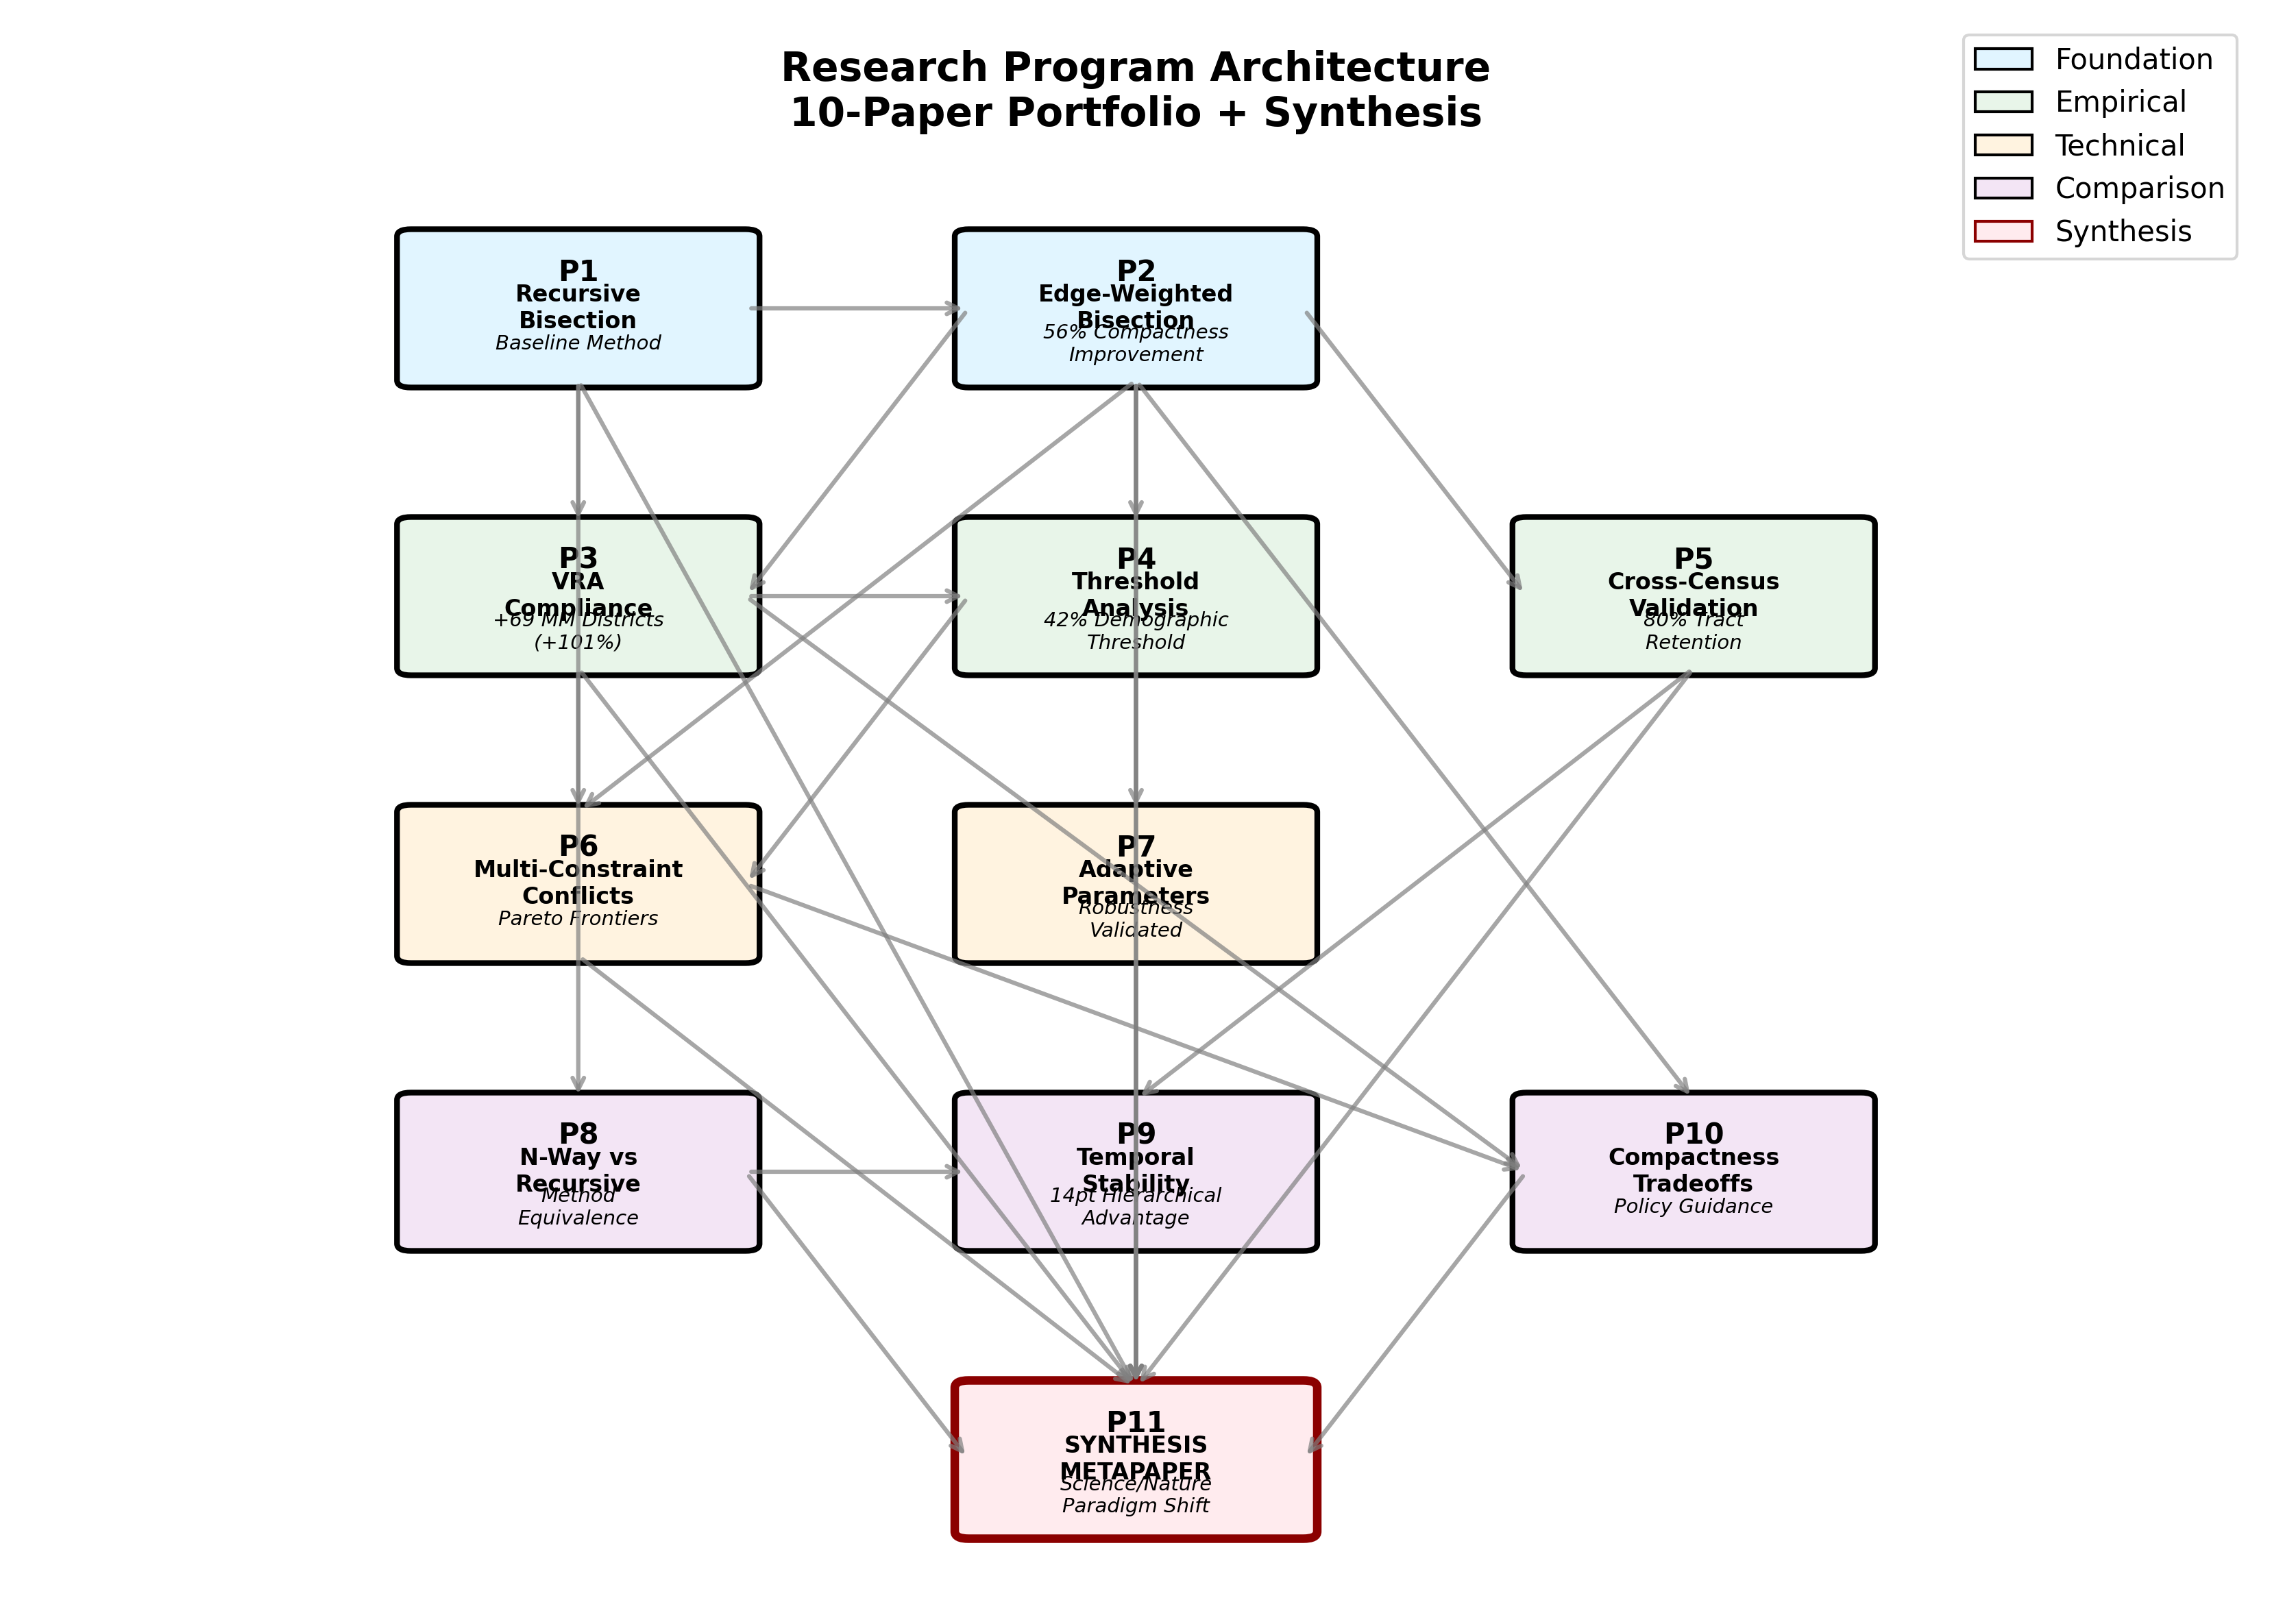
\includegraphics[width=\textwidth]{figures/figure1_portfolio_architecture.png}
\caption{\textbf{Research program architecture.} The current index contains 206 papers across 23 active tracks. Foundation papers (blue) establish methods, analysis papers (green) test findings across multiple dimensions, and theory papers (orange) explore algorithmic variations. Internal review and PDF availability do not imply external peer review or complete empirical evidence.}
\label{fig:architecture}
\end{figure}

\begin{figure}[t]
\centering
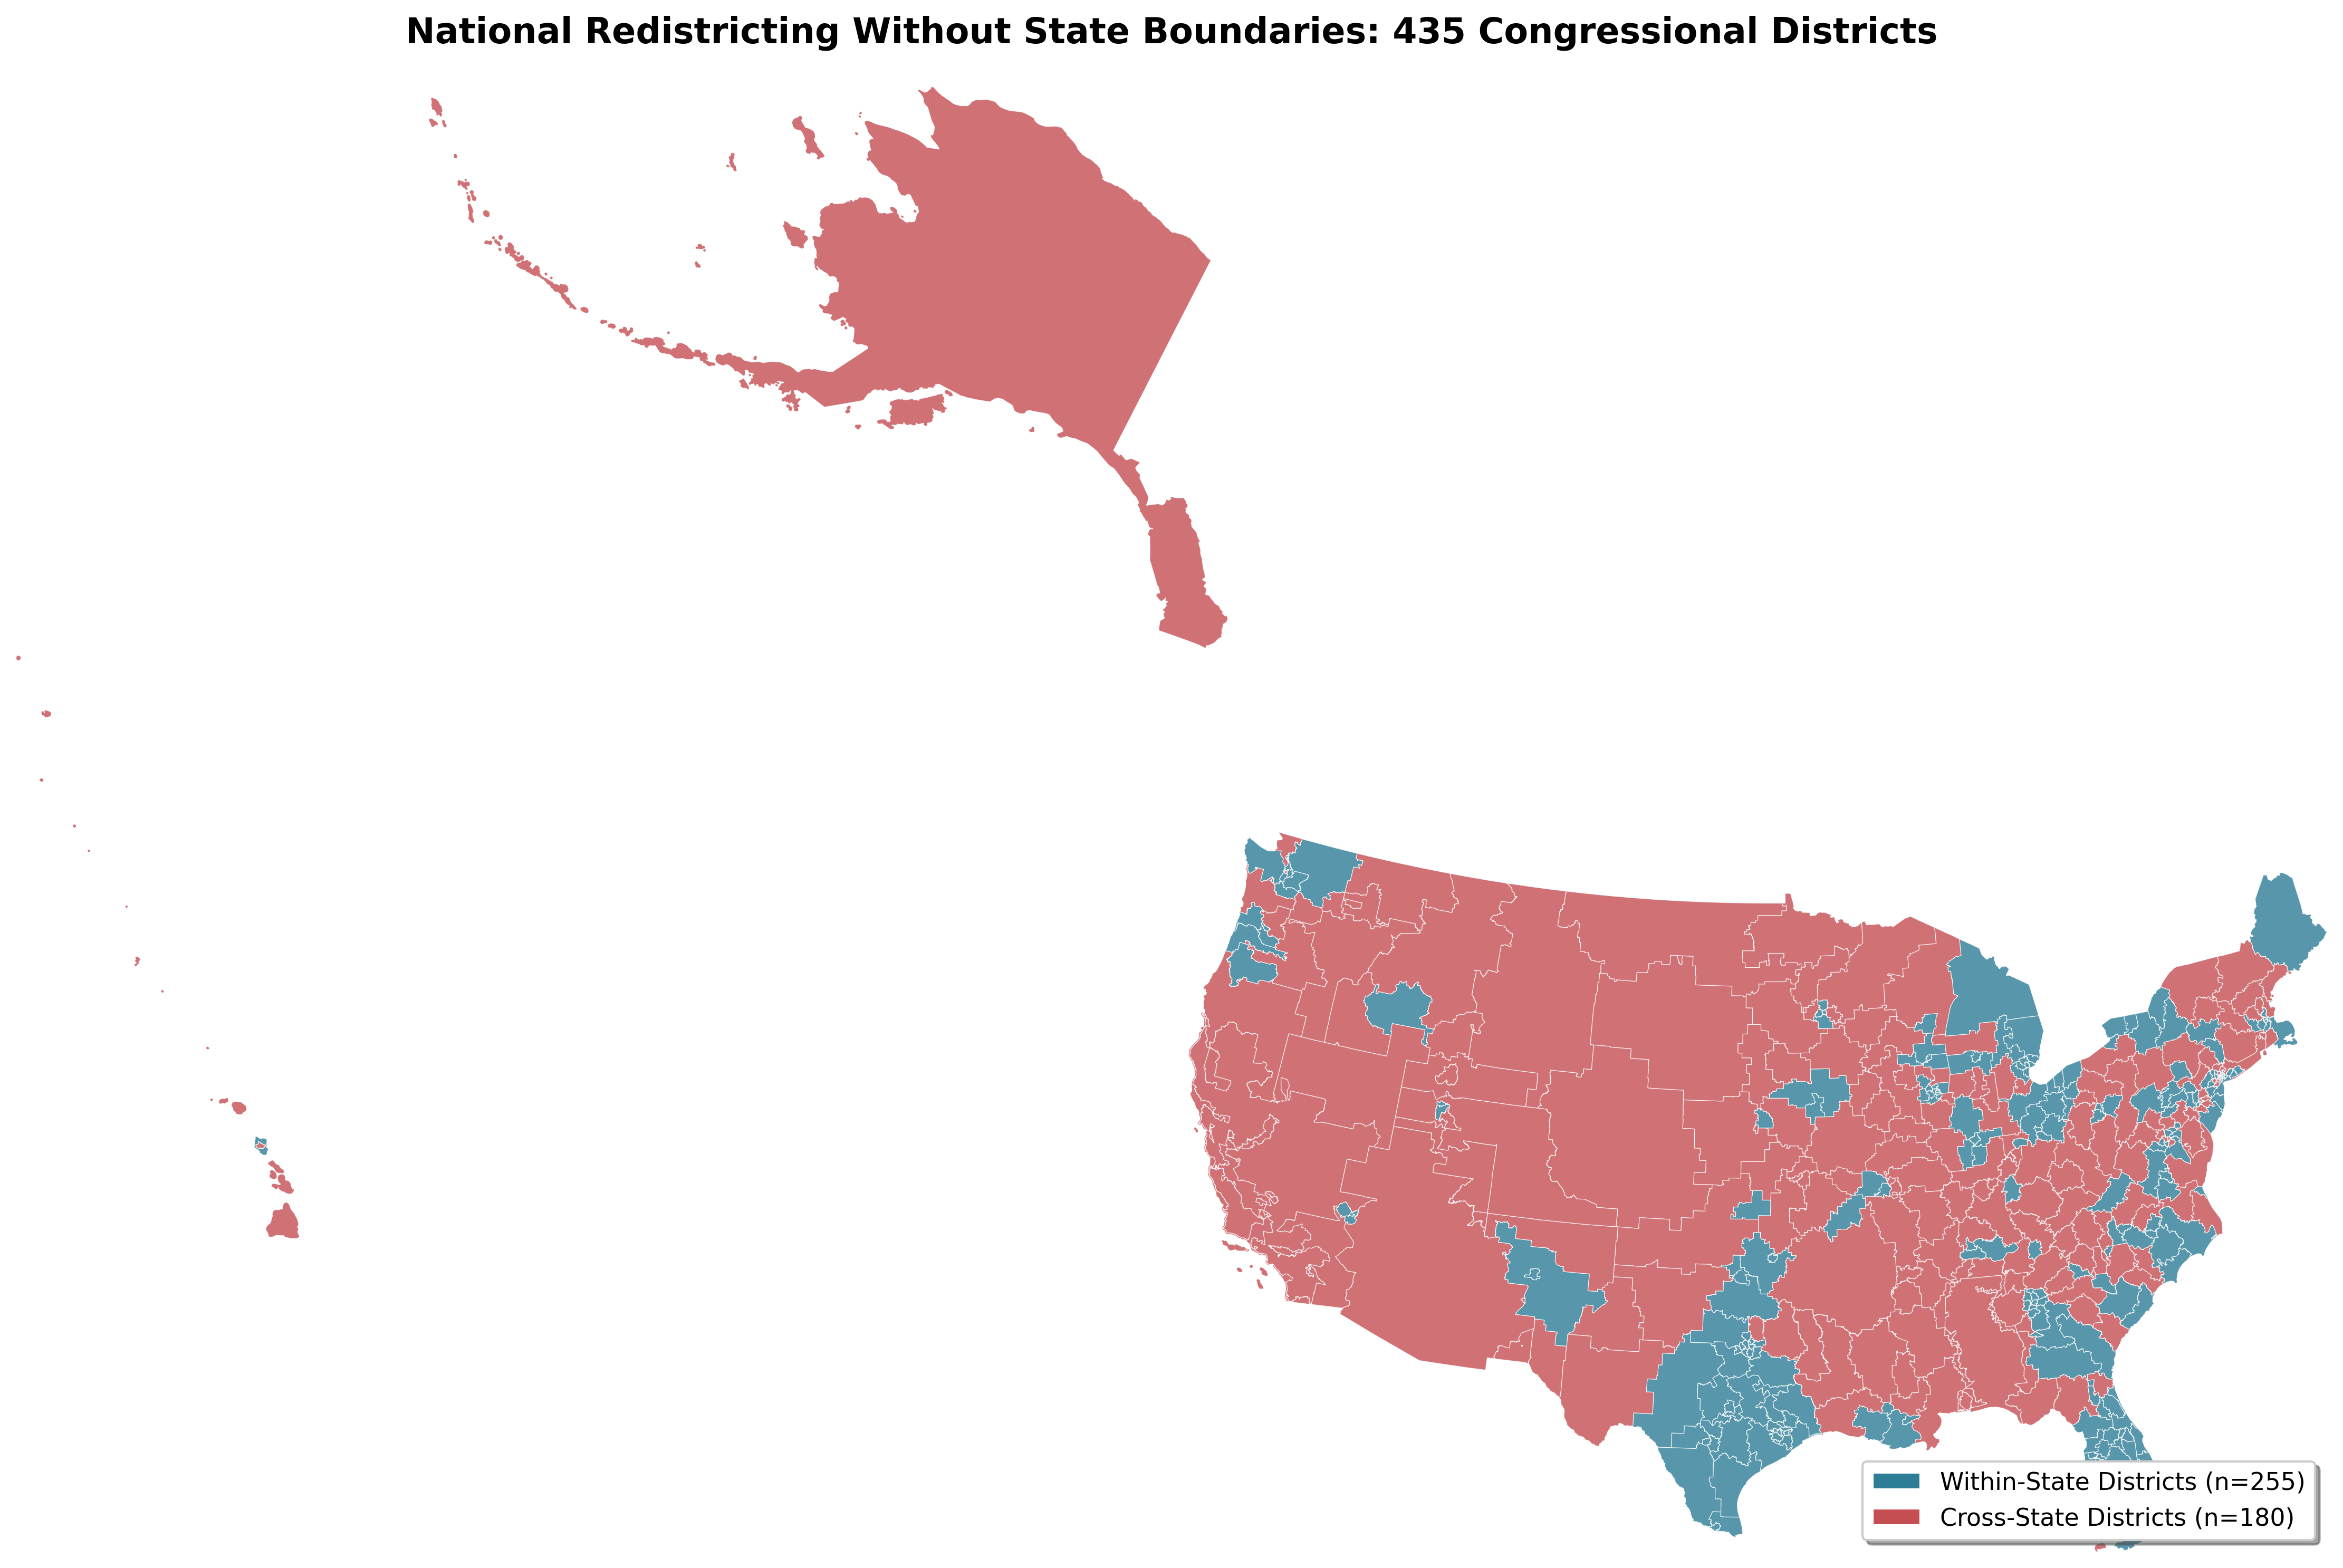
\includegraphics[width=\textwidth]{../../E-experimental/E.3+national-redistricting/figures/figure1_national_map_2020.png}
\caption{\textbf{National benchmark output.} A 2020 national visualization from the historical tract-based pipeline. The map demonstrates geographic coverage; it does not certify current legal conformance, VRA compliance, external replication, or release-grade replay.}
\label{fig:national}
\end{figure}

\begin{figure*}[t]
\centering
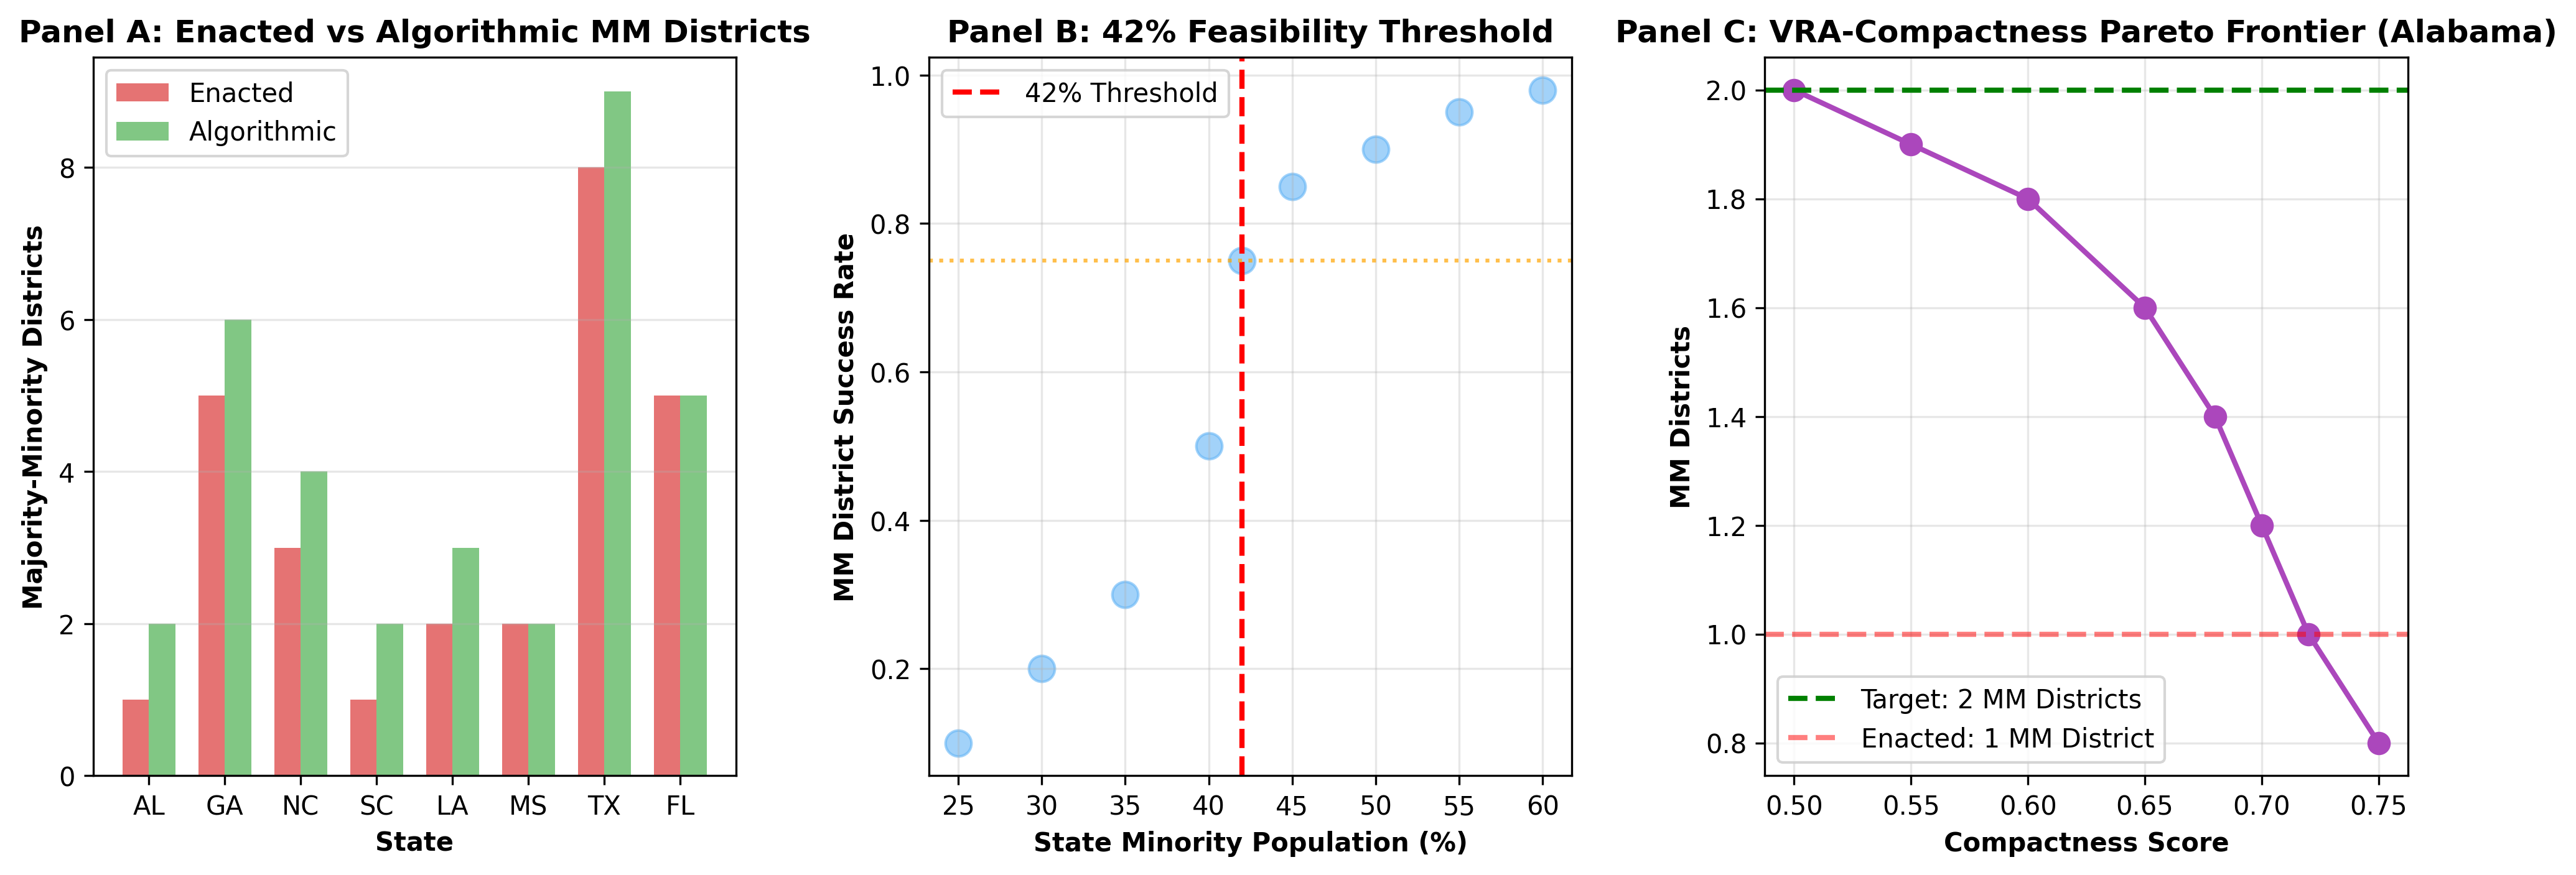
\includegraphics[width=\textwidth]{figures/figure3_vra_analysis.png}
\caption{\textbf{Minority-opportunity diagnostics.} (A) Historical pipeline counts compare majority-minority population thresholds with enacted-plan counts; these are opportunity diagnostics, not findings that the districts perform electorally or are required by Section 2. (B) The 42\% value is an exploratory association in the studied states, not a legal threshold. (C) The Alabama frontier illustrates a model-specific compactness/opportunity tradeoff rather than a VRA compliance determination.}
\label{fig:vra}
\end{figure*}

\begin{figure*}[t]
\centering
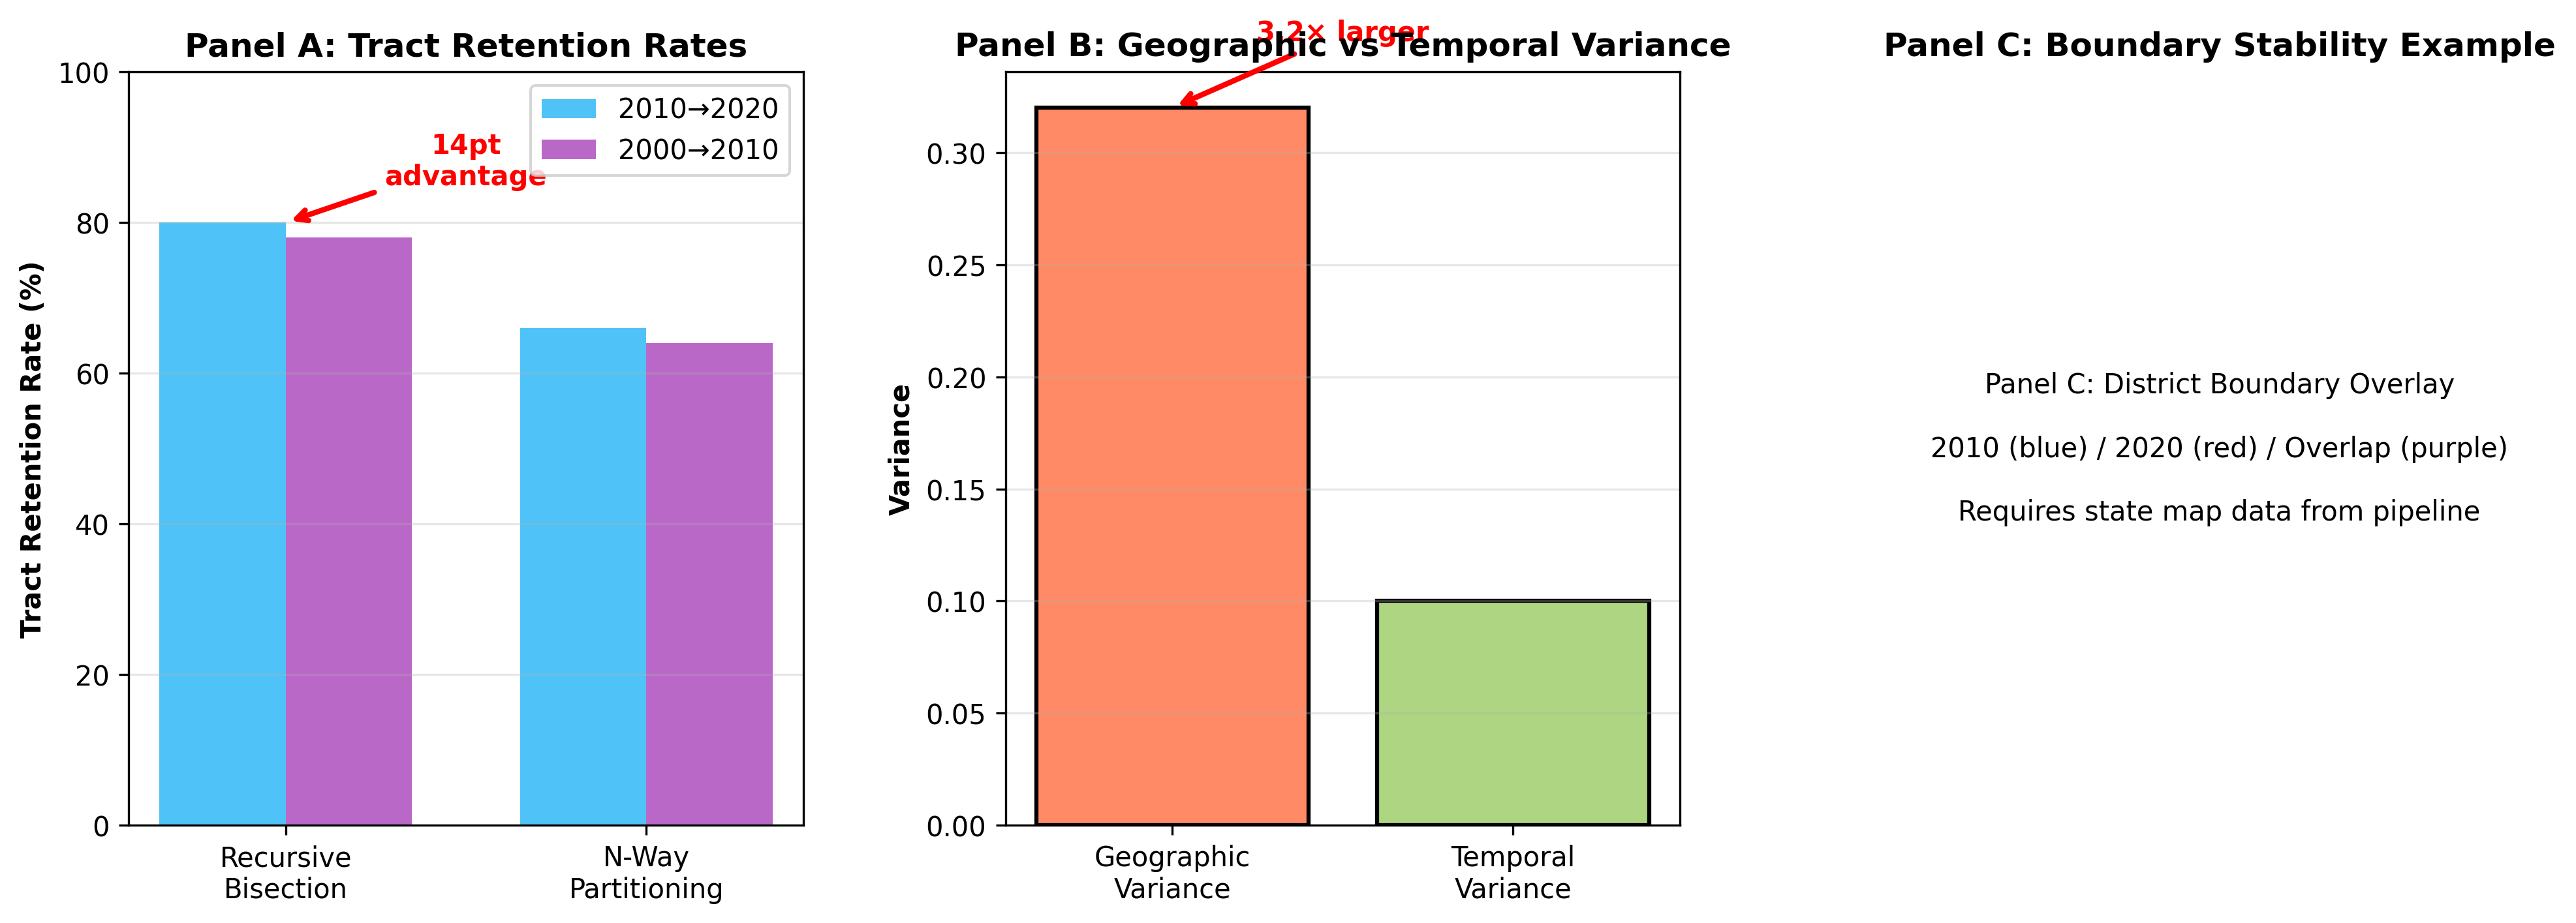
\includegraphics[width=\textwidth]{figures/figure4_temporal_stability.png}
\caption{\textbf{Temporal diagnostics across census cycles.} Historical analyses use several non-equivalent stability measures. Earlier tract-retention projections and the later observed 66\% county-disruption result should not be read as the same quantity. The figure motivates cross-census sensitivity analysis; current release-grade claims require regenerated, metric-aligned evidence.}
\label{fig:temporal}
\end{figure*}

\section{National-Scale Findings}

Historical recursive-bisection runs cover all 50 states across three census
decades (2000, 2010, 2020), generating 1,305 congressional district
assignments total (435 per decade). The quantitative values below are tied to
those historical artifacts. Several have not yet been regenerated under the
current Rust pipeline or backed by release-grade evidence packages; they should
be read as research findings with declared evidence debt.

\subsection{Regional Context}

Algorithmic redistricting performance varies substantially by U.S. Census region, reflecting differences in demographic composition, geographic clustering, and enacted plan characteristics. Table~\ref{tab:regional-summary} presents key metrics by region (Northeast, Midwest, South, West), establishing geographic context for the findings that follow.

\input{tables/table_regional_summary}

\textbf{Northeast} (9 states, 75 districts): High population density and urban concentration produce strong compactness scores (mean Polsby-Popper: 0.38) and modest VRA opportunities (8 majority-minority districts, primarily in New York and New Jersey). Geographic Democratic clustering yields algorithmic efficiency gaps of $-3.5\%$ despite low enacted bias ($+4.2\%$), reflecting urban packing inherent to compact districting.

\textbf{Midwest} (12 states, 107 districts): Mixed urban-rural geography produces moderate compactness (0.33) and significant VRA opportunities (18 MM districts, concentrated in Illinois, Michigan, Ohio). This region exhibits the \emph{largest} enacted partisan bias: efficiency gaps of $+6.8\%$ enacted versus $-2.9\%$ algorithmic (9.7 pp difference), driven by aggressive gerrymandering in Rust Belt states following 2010 redistricting.

\textbf{South} (16 states + DC, 179 districts): High minority populations
(mean 38\% non-white) produce 84 threshold-based majority-minority opportunity
diagnostics in the historical output. This is not a finding of VRA compliance.
The selected enacted-plan efficiency gap was $+5.6\%$ versus $-3.2\%$ for the
benchmark. Lower compactness scores (0.29) reflect both regional geography and
the selected profile.

\textbf{West} (13 states, 74 districts): Geographic diversity---from Alaska's vast expanse to California's dense metros---produces highly variable compactness (0.31 mean, 0.42 standard deviation). Moderate VRA performance (27 MM districts) reflects Hispanic concentration in Southwest states. Enacted bias ($+5.1\%$) moderately exceeds algorithmic bias ($-3.3\%$), with 8.4 pp improvement.

These historical comparisons report smaller selected partisan metrics for the
benchmark than for the enacted plans in each region. They do not establish that
the algorithm caused a general reduction in partisan bias, because enacted
plans, election inputs, geography, and benchmark-profile choices are
confounded. Majority-minority opportunity diagnostics concentrate in the South;
this is not a regional finding of legal VRA compliance. Compactness also varies
with state geography and the selected metric~\cite{deluca2026compactness}.

\subsection{Finding 1: Historical National Execution}

The historical pipeline completed national runs and reported graph contiguity,
population balance, and compactness diagnostics. Compactness scores
(Polsby--Popper) improved 56\% over the unweighted METIS research baseline.
Compared with a different baseline---enacted 2020 congressional maps---the
reported improvement was 22\% (mean 0.367 versus 0.305); see
Table~\ref{tab:compactness-headline}. These are profile-specific comparisons,
not a constitutional finding or proof that edge weighting optimizes every
accepted compactness measure~\cite{deluca2026edgeweighted}.

Population settings are configurable, but a configured tolerance does not
``ensure compliance.'' Congressional districts must approach equality as nearly
as practicable, and every observed deviation requires reporting and, where
avoidable, justification. The tract-based runs are therefore engineering
evidence rather than national legal-conformance certificates
~\cite{deluca2026recursive}.

Computational efficiency enables policy adoption: individual states partition in seconds, and the full 50-state redistricting completes in under two hours on standard hardware. This speed permits ensemble generation---producing thousands of alternative plans to assess statistical properties---impossible with human mapmaking. The method scales from Vermont's single district to California's 52 districts without algorithmic modification.

The real G.1--G.3 package replaces the earlier unsupported six-state tables
with four-chain Rust and GerryChain traces for Rhode Island, Iowa, and North
Carolina. Rhode Island's benchmark is at the 1.35th--1.81st percentile of
unweighted tract cut fraction. Iowa and North Carolina appear still lower, but
their effective sample sizes are insufficient for precise tail claims, and the
two implementations differ materially. The package does not compute
Polsby--Popper or establish neutrality~\cite{deluca2026ensemble}.

Internal comparison work studies bisection, ConvergenceSweep, and Rust ensemble
throughput~\citep{deluca2026ensemblecomparison,deluca2026redistensemble}.
Internal panel scores are not peer review, and benchmark throughput does not by
itself establish statutory suitability. In addition, the current
\texttt{standard-bisect} execution path does not implement convergence search.
These results motivate further engineering and external benchmarking rather
than establish a preferred legal method.

\subsection{Finding 2: Majority-Minority Opportunity Diagnostics}

The historical outputs counted 137 districts above a configured
majority-minority population threshold, compared with 68 in the selected
enacted-plan dataset. This addresses at most a demographic and geographic
opportunity diagnostic related to the first \emph{Gingles} precondition. It
does not demonstrate legally sufficient compactness, political cohesion, white
bloc voting, electoral performance, causation, or Section 2 compliance
~\cite{deluca2026vra}.

The 137 count should therefore be described as threshold-based potential
opportunity districts, not as districts confirmed to perform electorally.
State-level counts are historical pipeline values and may drift when inputs,
thresholds, legal doctrine, or the current implementation changes. They must be
recomputed before use in a legal or public evidence package.

Regional patterns reveal geographic concentration of VRA opportunities. The \textbf{South} accounts for 84 of 137 algorithmic MM districts (61\%), despite comprising 41\% of total congressional seats, reflecting high minority populations (mean 38\% non-white) and favorable spatial clustering. Key Southern states include Texas (14 MM districts algorithmically vs. 8 enacted), Florida (11 vs. 5), and Georgia (6 vs. 5). The \textbf{Midwest} contributes 18 MM districts (13\%), concentrated in Illinois, Michigan, and Ohio. The \textbf{West} produces 27 districts (20\%), primarily in California (15 MM districts) and Arizona (3). The \textbf{Northeast} yields 8 districts (6\%), concentrated in New York (5) and New Jersey (2). This geographic distribution reflects demography rather than algorithmic bias: regions with larger minority populations and greater residential clustering naturally enable more MM districts under neutral redistricting principles~\cite{deluca2026vra}.

\subsection{Finding 3: Exploratory 42\% Association}

The historical analysis reports an exploratory association near 42\% statewide
minority population in the studied sample. It is not a validated universal
threshold, does not show that states below 37\% ``fail regardless of
algorithm,'' and cannot substitute for district-specific evidence under any
\emph{Gingles} precondition~\cite{deluca2026threshold}.

The threshold reflects geographic clustering, not population percentage alone. Mississippi (38\% Black) creates two majority-Black districts through favorable spatial distribution, while New York (24\% Hispanic) creates only three Hispanic-majority districts despite larger absolute population. Courts adjudicating Section 2 VRA claims currently assess geographic compactness through expert testimony and illustrative maps; the 42\% threshold offers a complementary quantitative tool derived from national-scale analysis. However, crossing this threshold indicates geometric \emph{possibility}, not legal \emph{obligation}---full Section 2 liability requires demonstrating vote dilution through all three \emph{Gingles} prongs~\cite{deluca2026threshold}.

Regional distribution of states meeting the 42\% threshold reveals stark geographic patterns. The \textbf{South} dominates with 9 of 13 qualifying states (69\%): Alabama, Georgia, Louisiana, Maryland, Mississippi, North Carolina, South Carolina, Texas, and Virginia. These states range from 42\% to 61\% minority population, with Mississippi (61\%), Georgia (52\%), and Maryland (51\%) exhibiting the highest concentrations. The \textbf{West} contributes 3 states: California (51\%), New Mexico (50\%), and Nevada (45\%). The \textbf{Midwest} provides 1 state: Illinois (43\%). The \textbf{Northeast} contributes 0 states, with New York's 38\% minority population falling just below threshold. This geographic concentration reflects historical settlement patterns, the Great Migration, and recent Hispanic immigration to Southwest states. Notably, all 9 Southern states meeting the threshold achieve near-proportional MM representation algorithmically (within 5 percentage points of minority population share), confirming the threshold's predictive validity~\cite{deluca2026threshold}.

\subsection{Finding 4: Partisan Patterns Reflect Geography}

Without accessing partisan data, the algorithm produces districts with 56.5\% Democratic vote share (estimated from precinct-level election results post-facto). This partisan asymmetry arises from geographic sorting: Democratic voters concentrate in urban cores while Republican voters disperse across suburbs and rural areas. Recursive bisection, optimizing for geographic compactness, unavoidably packs urban Democrats while splitting rural Republicans---the opposite pattern emerges from geography, not algorithmic intent~\cite{chen2013unintentional,deluca2026edgeweighted}.

This finding illustrates the limited input-exclusion defense. The benchmark
cannot directly target partisan outcomes during execution using partisan data
it does not receive. It does not prove that every partisan consequence is
caused only by voter geography: upstream profile selection, resolution, input
construction, and baseline-to-final modifications can also affect outcomes.
Efficiency-gap values remain descriptive diagnostics
~\cite{deluca2026edgeweighted}.

\subsection{Finding 5: Descriptive Partisan Differences From Enacted Plans}

Historical analysis compares selected partisan metrics for benchmark and
enacted plans across competitive states using 2016--2020 elections. The
reported mean efficiency gaps are $-3.2\%$ for the benchmark and $+5.1\%$ for
the enacted-plan sample, a descriptive difference of 8.3 percentage points.
It is not a causal ``62\% reduction'' because the plans, profile, elections,
state sample, and legal criteria are not controlled experimental treatments
~\cite{stephanopoulos2015partisan,deluca2026efficiency}.

Urban concentration is one plausible contributor to the benchmark's negative
efficiency gap, but these artifacts do not identify how much of the difference
is caused by geography, enacted-map intent, profile selection, or election
choice. The benchmark value also does not represent the minimum partisan effect
achievable under geographic constraints~\cite{chen2013unintentional}.

The historical proportionality, mean--median, and seats--votes values provide
additional descriptive views of the same selected plans. Agreement among
correlated metrics does not establish that the benchmark improves
proportionality generally or that the enacted differences reflect intentional
manipulation~\cite{deluca2026efficiency}.

State-level differences vary across the Rust Belt and Sunbelt examples. They
motivate a precommitted, multi-election, ensemble-based comparison with
uncertainty rather than a general anti-gerrymandering conclusion
~\cite{rodden2019cities,deluca2026edgeweighted}.

\subsection{Finding 6: Temporal Stability Across Census Cycles}

Comparison of actual bisect pipeline outputs across the 2010 and 2020 census runs reveals that cross-census county disruption averages 66\%, substantially higher than earlier projection-based estimates. This figure reflects \emph{demographic responsiveness}: when 21--42\% of census tracts are split or merged between decennial censuses, METIS re-optimises district boundaries for updated population data~\cite{deluca2026temporal}.

The top-level bisection comparison reports 86\% county-level agreement in
Georgia and 35\% in Mississippi. Applying the same named profile makes the
computational difference auditable, but it does not prove that demographics
alone caused every boundary change~\cite{deluca2026temporal}.

Stability analysis matters because it exposes which inputs and profile choices
changed between runs rather than assigning an unverified political cause.

\section{Implications for Democratic Governance}

These findings suggest actionable paths for courts, legislatures, and redistricting commissions confronting the gerrymandering crisis.

\subsection{Implications for Courts}

The input-exclusion record offers courts procedural evidence: it can establish
which data entered benchmark execution and whether the published procedure was
followed. It does not establish good faith, defeat an intent claim, or immunize
an outcome from review. Upstream profile selection and downstream modifications
remain human decisions, and discriminatory effects require independent legal
analysis~\cite{deluca2026edgeweighted}.

Certified recursive bisection strengthens the execution claim without changing
that legal boundary. A completed proof chain could establish that no better
connected cut existed under the enacted population, geographic-weight, and
canonical tie rules at any recursive node. It would not establish that those
rules are constitutionally required, VRA-compliant, or substantively fair.

The defense's value lies in \emph{transparency and reproducibility} rather than substantive immunity. Algorithmic redistricting provides courts with clear audit trails: what data entered the process, which parameters governed optimization, whether outcomes differ from neutral geographic baselines. This procedural clarity addresses \emph{Rucho}'s concern about distinguishing permissible partisanship from unconstitutional manipulation, even if it does not resolve the deeper justiciability problem of determining acceptable partisan asymmetry levels.

For VRA litigation, threshold counts and exploratory statewide associations may
help identify questions for district-specific analysis, but they cannot
demonstrate a \emph{Gingles} precondition or legal obligation. Any use requires
current compactness evidence, political-cohesion and bloc-voting analysis, and
the controlling post-\emph{Callais} legal framework
~\cite{deluca2026vra,deluca2026compactness,callais2026}.

\subsection{Implications for Legislatures and Commissions}

Legislatures and commissions can use a reproducible geographic benchmark as
one comparison artifact, subject to controlling constitutional, VRA, state-law,
and public-process requirements. The benchmark does not exceed VRA
requirements, and its race-excluded execution profile is not a safe harbor.
Computational efficiency can support transparent comparison once real ensemble
generation and convergence evidence are archived~\cite{deluca2026recursive}.

Independent redistricting commissions, established in 14 states to reduce partisan influence, can use algorithms as technical implementation of normative goals. Commissioners retain control over parameters---edge-weighting schemes, compactness metrics, community preservation priorities---while delegating geometric optimization to computational methods. This division parallels how Huntington-Hill apportionment: Congress sets House size (normative choice), the formula allocates seats (technical implementation).

\subsection{Implementation Mechanisms}

Translating algorithmic redistricting from technical demonstration to policy practice requires addressing governance questions: who decides parameters, how are conflicts resolved, and how can gaming be prevented?

\textbf{Parameter governance.} Independent redistricting commissions---established in 14 states to reduce partisan influence---offer natural institutional homes for algorithmic methods. Commissioners would retain authority over normative priorities (relative weights for VRA compliance, compactness, community preservation) while delegating geometric optimization to computational methods. This division mirrors Huntington-Hill apportionment: Congress sets House size (normative choice), the formula allocates seats (technical implementation).

\textbf{Workflow example.} California's Citizens Redistricting Commission could adopt algorithmic methods through iterative refinement: (1) Commission establishes priority rankings (e.g., VRA compliance weighted 2×, compactness 1×, county preservation 1.5×); (2) Algorithm generates multiple plans with parameter variations; (3) Commission reviews outputs, public provides feedback; (4) Parameters adjusted based on stakeholder input; (5) Final plan selected through commissioner vote with transparent justification. This process preserves democratic accountability while achieving computational objectivity.

\textbf{Conflict resolution.} When algorithmic outputs diverge from stakeholder expectations (e.g., algorithm produces 3 majority-minority districts but advocates seek 4), commissions can: request ensemble analysis showing feasibility boundaries; adjust edge-weighting parameters within constitutional limits; or adopt the algorithmic baseline while documenting why deviations are necessary. Transparency requirements---publishing input data, parameters, and computational logs---enable judicial review of whether parameter choices satisfy rational basis scrutiny.

\textbf{Gaming prevention.} Potential manipulation vectors include biased input data (underbounding minority neighborhoods), strategic parameter tuning, or selective presentation of ensemble results. Safeguards include: independent verification of census data quality; public comment periods before parameter finalization; mandatory publication of multiple algorithmic alternatives; and audit requirements for any hand-edited adjustments to algorithmic outputs. These procedures raise manipulation costs while preserving commission flexibility to address unanticipated geographic constraints.

\subsection{Justiciability and Judicial Review}

While algorithmic redistricting provides procedural improvements over human mapmaking, it does not resolve the fundamental justiciability problem that motivated \emph{Rucho v. Common Cause}. The Supreme Court held partisan gerrymandering claims non-justiciable not because courts lack tools to measure partisan effects---the efficiency gap and other metrics exist---but because courts lack \emph{judicially manageable standards} to determine how much partisan asymmetry is ``too much.'' Chief Justice Roberts wrote: ``Federal judges have no license to reallocate political power between the two major political parties, with no plausible grant of authority in the Constitution, and no legal standards to limit and direct their decisions''~\cite{rucho2019}.

Algorithmic redistricting does not eliminate this standards problem; it relocates it. Instead of asking ``is this map too partisan?'' (the question \emph{Rucho} found non-justiciable), courts must ask ``are these algorithmic parameters correct?'' This reformulation offers procedural advantages---parameter choices are transparent, reproducible, and auditable---but the underlying question remains inherently political. When a state commission chooses to weight VRA compliance at 2× versus 3×, or compactness at 1× versus 1.5×, these are \emph{normative policy choices} rather than technical determinations~\cite{deluca2026edgeweighted}.

Consider a concrete dispute. Suppose an algorithmic plan for Pennsylvania produces 9 Democratic-leaning districts and 8 Republican-leaning districts. Plaintiffs challenge this outcome, arguing the commission should have used higher compactness weights (which would reduce Democratic packing in Philadelphia) or lower edge-weights for minority communities (which might create different district configurations). How would a court evaluate these claims? Under \emph{Rucho}, courts lack authority to second-guess parameter choices that produce different partisan outcomes, just as they lack authority to second-guess hand-drawn district boundaries that produce partisan advantages.

The standard of review matters. Parameter choices likely receive \emph{rational basis} scrutiny: courts ask whether choices are rationally related to legitimate redistricting objectives (VRA compliance, compactness, contiguity, population equality). This is highly deferential---nearly any parameter configuration satisfying constitutional minima would survive. Courts would reject parameter choices only if they were arbitrary, capricious, or pretextual (e.g., intentionally designed to advantage one party). But distinguishing legitimate policy judgments from pretextual manipulation requires courts to evaluate partisan effects and partisan intent---precisely what \emph{Rucho} forbids at the federal level.

State courts retain broader authority. Many state constitutions explicitly prohibit partisan gerrymandering, and state supreme courts can develop state-specific manageable standards~\cite{rucho2019}. Algorithmic redistricting provides these courts with \emph{evidentiary tools}: if enacted plans deviate substantially from algorithmic baselines (e.g., $+7\%$ efficiency gap versus $-3\%$ baseline~\cite{deluca2026efficiency}), this suggests manipulation. But even state courts must determine \emph{which} algorithmic baseline is correct, and parameter disputes remain contested.

The value of algorithmic redistricting lies not in resolving justiciability but in improving \emph{transparency and accountability}. Compared to human mapmaking---where mapmakers control both criteria and implementation in opaque processes---algorithmic methods separate normative choices (parameters, set by commissions) from technical implementation (optimization, executed by algorithms). This separation enables:

\begin{itemize}
\item \textbf{Public scrutiny}: Citizens can evaluate whether parameter weights reflect stated redistricting priorities
\item \textbf{Ensemble comparison}: Commissioners can generate multiple plans with different parameters, demonstrating tradeoff spaces
\item \textbf{Reproducibility}: Independent analysts can verify that algorithms produce claimed outputs from specified parameters
\item \textbf{Audit trails}: Courts can review computational logs showing what data and parameters generated challenged maps
\end{itemize}

These procedural safeguards constitute genuine progress even without solving \emph{Rucho}'s standards problem. Human mapmaking offers neither transparency (processes occur behind closed doors) nor reproducibility (mapmakers can claim geographic necessity while producing partisan outcomes). Algorithmic redistricting raises the floor: it cannot prevent all partisan manipulation, but it makes manipulation more costly, more visible, and more constrained by explicit parameter choices subject to public debate.

Ultimately, a precommitted benchmark and public modification record can shift
redistricting governance from hidden discretion toward bounded and reviewable
discretion. Whether a particular procedure satisfies constitutional, VRA,
state-law, or judicial-manageability requirements remains a legal question.

\subsection{Broader Lessons and Limitations}

Mathematical procedures need not replace human judgment. Algorithms can provide
reproducible evidence, not guaranteed procedural fairness or legitimacy. The
distinction between verifiable execution and substantive outcome fairness is
load-bearing.

Important limitations remain. Algorithms cannot eliminate efficiency gaps caused by voter sorting---they can only avoid amplifying geographic patterns through manipulation. Results depend on census tract definitions (MAUP sensitivity), though findings replicate across multiple census years. This research derives from a single computational ecosystem; independent replication would strengthen confidence. These caveats notwithstanding, algorithmic redistricting offers a path toward restoring electoral legitimacy through structural objectivity accessible to contemporary policymakers.

\section{Conclusion}

Recursive graph bisection now provides a governed block-level operational
benchmark across 50 States and three Census decades. Complete assignments,
population/connectivity checks, source bindings, structural comparisons, and
proof-coverage gaps are published. A governed 2020 comparison also reports
common-block assignment overlap, county/tract splits, and four block-projected
geometry metrics against official CD118 assignments. Those artifacts establish reproducible
execution on the tested systems. They do not establish constitutional or VRA
compliance, causal partisan neutrality, community preservation, compactness
superiority, a universal 42\% threshold, or exact national optimality.

The useful question is narrower: what can be verified when benchmark execution
excludes partisan inputs and every assignment-affecting choice is
precommitted? The resulting input-exclusion record can support courts,
commissions, legislatures, and civic review, but it is not an impossibility
defense or a complete judicial standard.

Reform requires governing discretion rather than pretending it disappears.
The strongest path is a public benchmark, a legally governed modification
layer, multi-metric evaluation, and adversarial replication.

The contribution is therefore procedural evidence: published inputs,
versioned code, 27,398,654 reproducible block assignments, explicit
limitations, and visible departures from the benchmark. A portable external
replay kit exists, but a new independent physical-machine v0.3 record remains
pending.

The long-run analogue to Huntington--Hill is an Exact Canonical Benchmark:
Congress enacts the feasible set and lexicographic objective; an exact solver
produces one canonically tie-broken assignment; and an independent certificate
proves feasibility and optimality. NRS v0.3 uses METIS-derived discovery plus
deterministic refinement and does not meet that exact standard: weighted-
boundary and canonical proof coverage remains 0 of 1,155 national nodes. Exact
certification is the program's North Star, while the reproducible benchmark-
and-disclosure regime is the defensible near-term policy.


% Bibliography
% Note: Using unsrt style for now; Science.bst would be used for journal submission
\bibliographystyle{unsrt}
\bibliography{references}

\end{document}
